\pc{2}{3/2}

\question Convert each of the following regular expressions
into an equivalent NFA.
Recall that $^\star$ has highest precedence,
then concatenation, then $\mid$.
For example,
$ab \mid abc^\star$
is interpreted as
$(ab) \mid (ab(c^\star))$.
Similarly,
$a\mid b^\star$
is equivalent to
$(a) \mid (b^\star)$.
\begin{parts}
    \part $ab^\star c$;
    \begin{solution}
        \begin{center}
            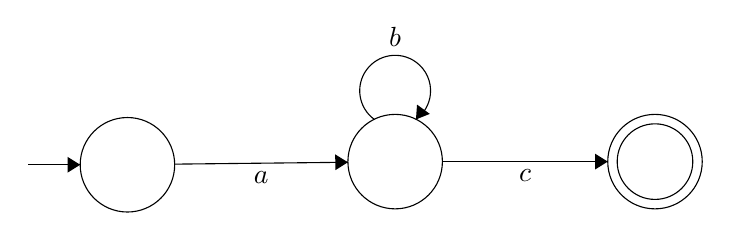
\begin{tikzpicture}[scale=0.2]
                \tikzstyle{every node}+=[inner sep=0pt]
                \draw [black] (9.7,-19.8) circle (3);
                \draw [black] (26.7,-19.6) circle (3);
                \draw [black] (43.2,-19.6) circle (3);
                \draw [black] (43.2,-19.6) circle (2.4);
                \draw [black] (3.4,-19.8) -- (6.7,-19.8);
                \fill [black] (6.7,-19.8) -- (5.9,-19.3) -- (5.9,-20.3);
                \draw [black] (12.7,-19.76) -- (23.7,-19.64);
                \fill [black] (23.7,-19.64) -- (22.89,-19.14) -- (22.91,-20.14);
                \draw (18.2,-20.21) node [below] {$a$};
                \draw [black] (25.377,-16.92) arc (234:-54:2.25);
                \draw (26.7,-12.35) node [above] {$b$};
                \fill [black] (28.02,-16.92) -- (28.9,-16.57) -- (28.09,-15.98);
                \draw [black] (29.7,-19.6) -- (40.2,-19.6);
                \fill [black] (40.2,-19.6) -- (39.4,-19.1) -- (39.4,-20.1);
                \draw (34.95,-20.1) node [below] {$c$};
            \end{tikzpicture}
        \end{center}
    \end{solution}

    \part $(a \mid b)^\star abb$;
    \begin{solution}
        \begin{center}
            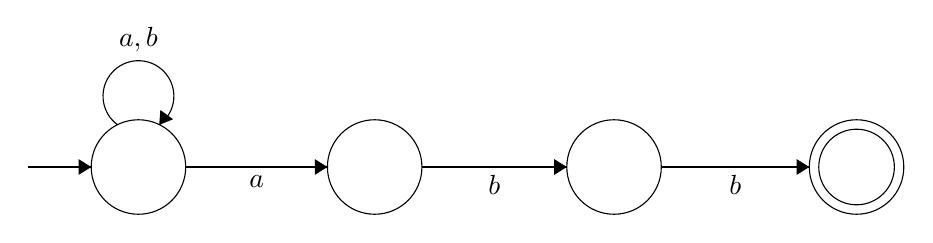
\begin{tikzpicture}[scale=0.2]
                \tikzstyle{every node}+=[inner sep=0pt]
                \draw [black] (10.3,-21.9) circle (3);
                \draw [black] (25.3,-21.9) circle (3);
                \draw [black] (40.5,-21.9) circle (3);
                \draw [black] (55.9,-21.9) circle (3);
                \draw [black] (55.9,-21.9) circle (2.4);
                \draw [black] (3.3,-21.9) -- (7.3,-21.9);
                \fill [black] (7.3,-21.9) -- (6.5,-21.4) -- (6.5,-22.4);
                \draw [black] (8.977,-19.22) arc (234:-54:2.25);
                \draw (10.3,-14.65) node [above] {$a,b$};
                \fill [black] (11.62,-19.22) -- (12.5,-18.87) -- (11.69,-18.28);
                \draw [black] (13.3,-21.9) -- (22.3,-21.9);
                \fill [black] (22.3,-21.9) -- (21.5,-21.4) -- (21.5,-22.4);
                \draw (17.8,-22.4) node [below] {$a$};
                \draw [black] (28.3,-21.9) -- (37.5,-21.9);
                \fill [black] (37.5,-21.9) -- (36.7,-21.4) -- (36.7,-22.4);
                \draw (32.9,-22.4) node [below] {$b$};
                \draw [black] (43.5,-21.9) -- (52.9,-21.9);
                \fill [black] (52.9,-21.9) -- (52.1,-21.4) -- (52.1,-22.4);
                \draw (48.2,-22.4) node [below] {$b$};
            \end{tikzpicture}
        \end{center}
    \end{solution}

    \part $(a \mid c)^\star b (a \mid c)^\star b (a \mid c)^\star$;
    \begin{solution}
        \begin{center}
            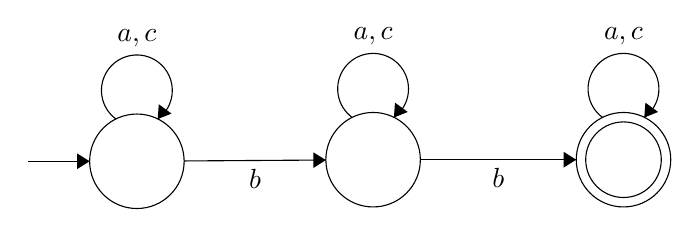
\begin{tikzpicture}[scale=0.2]
                \tikzstyle{every node}+=[inner sep=0pt]
                \draw [black] (17.1,-25.8) circle (3);
                \draw [black] (32.1,-25.7) circle (3);
                \draw [black] (48,-25.7) circle (3);
                \draw [black] (48,-25.7) circle (2.4);
                \draw [black] (10.2,-25.8) -- (14.1,-25.8);
                \fill [black] (14.1,-25.8) -- (13.3,-25.3) -- (13.3,-26.3);
                \draw [black] (15.777,-23.12) arc (234:-54:2.25);
                \draw (17.1,-18.55) node [above] {$a,c$};
                \fill [black] (18.42,-23.12) -- (19.3,-22.77) -- (18.49,-22.18);
                \draw [black] (20.1,-25.78) -- (29.1,-25.72);
                \fill [black] (29.1,-25.72) -- (28.3,-25.23) -- (28.3,-26.23);
                \draw (24.6,-26.26) node [below] {$b$};
                \draw [black] (30.777,-23.02) arc (234:-54:2.25);
                \draw (32.1,-18.45) node [above] {$a,c$};
                \fill [black] (33.42,-23.02) -- (34.3,-22.67) -- (33.49,-22.08);
                \draw [black] (35.1,-25.7) -- (45,-25.7);
                \fill [black] (45,-25.7) -- (44.2,-25.2) -- (44.2,-26.2);
                \draw (40.05,-26.2) node [below] {$b$};
                \draw [black] (46.677,-23.02) arc (234:-54:2.25);
                \draw (48,-18.45) node [above] {$a,c$};
                \fill [black] (49.32,-23.02) -- (50.2,-22.67) -- (49.39,-22.08);
            \end{tikzpicture}
        \end{center}
    \end{solution}

    \part $a^\star (\varepsilon \mid ab (a \mid b \mid c)^\star)$; and
    \begin{solution}
        \begin{center}
            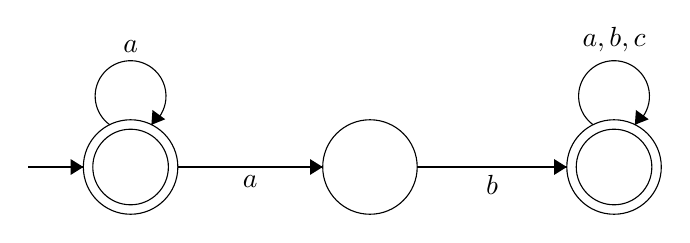
\begin{tikzpicture}[scale=0.2]
                \tikzstyle{every node}+=[inner sep=0pt]
                \draw [black] (14.1,-22.2) circle (3);
                \draw [black] (14.1,-22.2) circle (2.4);
                \draw [black] (29.3,-22.2) circle (3);
                \draw [black] (44.8,-22.2) circle (3);
                \draw [black] (44.8,-22.2) circle (2.4);
                \draw [black] (7.6,-22.2) -- (11.1,-22.2);
                \fill [black] (11.1,-22.2) -- (10.3,-21.7) -- (10.3,-22.7);
                \draw [black] (12.777,-19.52) arc (234:-54:2.25);
                \draw (14.1,-14.95) node [above] {$a$};
                \fill [black] (15.42,-19.52) -- (16.3,-19.17) -- (15.49,-18.58);
                \draw [black] (17.1,-22.2) -- (26.3,-22.2);
                \fill [black] (26.3,-22.2) -- (25.5,-21.7) -- (25.5,-22.7);
                \draw (21.7,-22.7) node [below] {$a$};
                \draw [black] (32.3,-22.2) -- (41.8,-22.2);
                \fill [black] (41.8,-22.2) -- (41,-21.7) -- (41,-22.7);
                \draw (37.05,-22.7) node [below] {$b$};
                \draw [black] (43.477,-19.52) arc (234:-54:2.25);
                \draw (44.8,-14.95) node [above] {$a,b,c$};
                \fill [black] (46.12,-19.52) -- (47,-19.17) -- (46.19,-18.58);
            \end{tikzpicture}
        \end{center}
    \end{solution}

    \part $(10) \mid (10^\star 1)$.
    \begin{solution}
        \begin{center}
            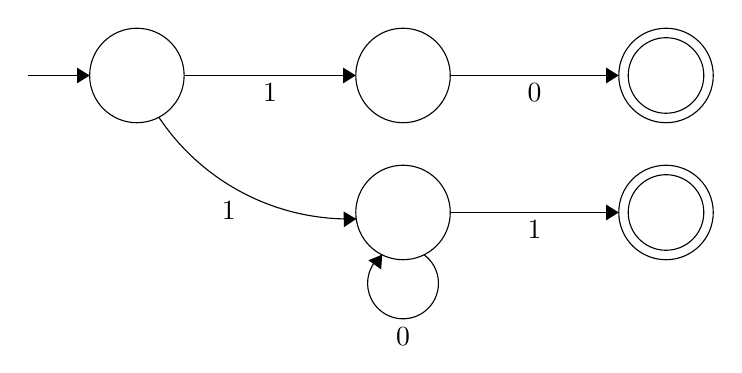
\begin{tikzpicture}[scale=0.2]
                \tikzstyle{every node}+=[inner sep=0pt]
                \draw [black] (12.1,-22.3) circle (3);
                \draw [black] (29,-22.3) circle (3);
                \draw [black] (45.7,-22.3) circle (3);
                \draw [black] (45.7,-22.3) circle (2.4);
                \draw [black] (29,-31) circle (3);
                \draw [black] (45.7,-31) circle (3);
                \draw [black] (45.7,-31) circle (2.4);
                \draw [black] (5.2,-22.3) -- (9.1,-22.3);
                \fill [black] (9.1,-22.3) -- (8.3,-21.8) -- (8.3,-22.8);
                \draw [black] (15.1,-22.3) -- (26,-22.3);
                \fill [black] (26,-22.3) -- (25.2,-21.8) -- (25.2,-22.8);
                \draw (20.55,-22.8) node [below] {$1$};
                \draw [black] (32,-22.3) -- (42.7,-22.3);
                \fill [black] (42.7,-22.3) -- (41.9,-21.8) -- (41.9,-22.8);
                \draw (37.35,-22.8) node [below] {$0$};
                \draw [black] (26.033,-31.405) arc (-88.14659:-146.33159:14.503);
                \fill [black] (26.03,-31.41) -- (25.22,-30.93) -- (25.25,-31.93);
                \draw (17.93,-30.31) node [below] {$1$};
                \draw [black] (30.323,-33.68) arc (54:-234:2.25);
                \draw (29,-38.25) node [below] {$0$};
                \fill [black] (27.68,-33.68) -- (26.8,-34.03) -- (27.61,-34.62);
                \draw [black] (32,-31) -- (42.7,-31);
                \fill [black] (42.7,-31) -- (41.9,-30.5) -- (41.9,-31.5);
                \draw (37.35,-31.5) node [below] {$1$};
            \end{tikzpicture}
        \end{center} 
    \end{solution}
\end{parts}

\question Consider the following NFA over the alpabet
$\{a,b,c\}$:
\begin{center}
    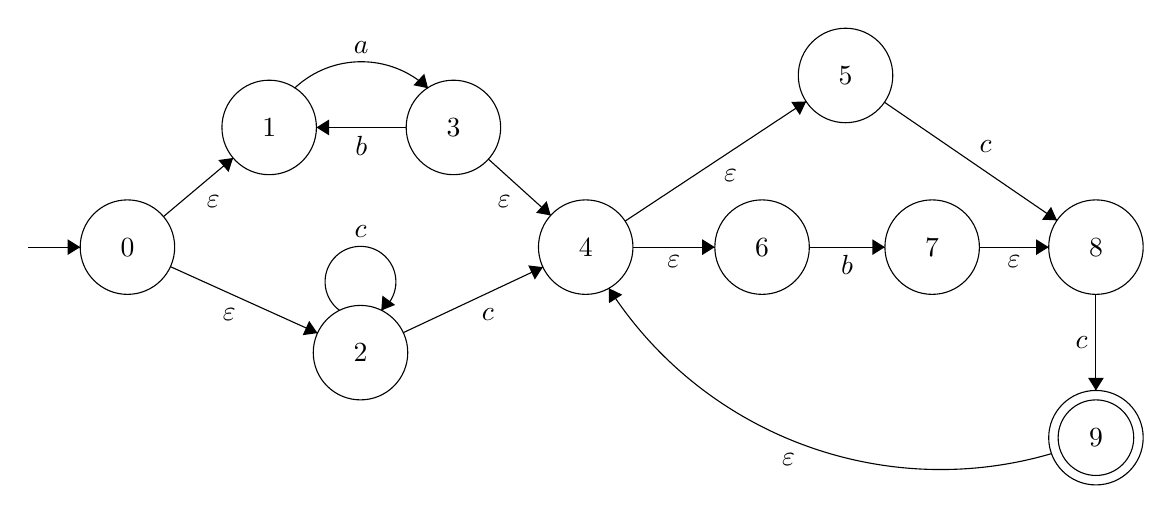
\begin{tikzpicture}[scale=0.2]
        \tikzstyle{every node}+=[inner sep=0pt]
        \draw [black] (8.7,-27.8) circle (3);
        \draw (8.7,-27.8) node {$0$};
        \draw [black] (17.7,-20.2) circle (3);
        \draw (17.7,-20.2) node {$1$};
        \draw [black] (29.4,-20.2) circle (3);
        \draw (29.4,-20.2) node {$3$};
        \draw [black] (23.5,-34.5) circle (3);
        \draw (23.5,-34.5) node {$2$};
        \draw [black] (37.8,-27.8) circle (3);
        \draw (37.8,-27.8) node {$4$};
        \draw [black] (49,-27.8) circle (3);
        \draw (49,-27.8) node {$6$};
        \draw [black] (54.3,-16.9) circle (3);
        \draw (54.3,-16.9) node {$5$};
        \draw [black] (59.8,-27.8) circle (3);
        \draw (59.8,-27.8) node {$7$};
        \draw [black] (70.2,-27.8) circle (3);
        \draw (70.2,-27.8) node {$8$};
        \draw [black] (70.2,-39.9) circle (3);
        \draw (70.2,-39.9) node {$9$};
        \draw [black] (70.2,-39.9) circle (2.4);
        \draw [black] (2.4,-27.8) -- (5.7,-27.8);
        \fill [black] (5.7,-27.8) -- (4.9,-27.3) -- (4.9,-28.3);
        \draw [black] (10.99,-25.86) -- (15.41,-22.14);
        \fill [black] (15.41,-22.14) -- (14.47,-22.27) -- (15.12,-23.03);
        \draw (14.15,-24.49) node [below] {$\varepsilon$};
        \draw [black] (11.43,-29.04) -- (20.77,-33.26);
        \fill [black] (20.77,-33.26) -- (20.24,-32.48) -- (19.83,-33.39);
        \draw (15.17,-31.66) node [below] {$\varepsilon$};
        \draw [black] (19.313,-17.705) arc (133.22493:46.77507:6.187);
        \fill [black] (27.79,-17.71) -- (27.55,-16.79) -- (26.86,-17.52);
        \draw (23.55,-15.53) node [above] {$a$};
        \draw [black] (26.4,-20.2) -- (20.7,-20.2);
        \fill [black] (20.7,-20.2) -- (21.5,-20.7) -- (21.5,-19.7);
        \draw (23.55,-20.7) node [below] {$b$};
        \draw [black] (22.177,-31.82) arc (234:-54:2.25);
        \draw (23.5,-27.25) node [above] {$c$};
        \fill [black] (24.82,-31.82) -- (25.7,-31.47) -- (24.89,-30.88);
        \draw [black] (26.22,-33.23) -- (35.08,-29.07);
        \fill [black] (35.08,-29.07) -- (34.15,-28.96) -- (34.57,-29.86);
        \draw (31.58,-31.66) node [below] {$c$};
        \draw [black] (31.62,-22.21) -- (35.58,-25.79);
        \fill [black] (35.58,-25.79) -- (35.32,-24.88) -- (34.65,-25.62);
        \draw (32.64,-24.49) node [below] {$\varepsilon$};
        \draw [black] (40.8,-27.8) -- (46,-27.8);
        \fill [black] (46,-27.8) -- (45.2,-27.3) -- (45.2,-28.3);
        \draw (43.4,-28.3) node [below] {$\varepsilon$};
        \draw [black] (40.3,-26.15) -- (51.8,-18.55);
        \fill [black] (51.8,-18.55) -- (50.85,-18.58) -- (51.4,-19.41);
        \draw (47,-22.85) node [below] {$\varepsilon$};
        \draw [black] (67.378,-40.913) arc (-73.68447:-147.2725:25.05);
        \fill [black] (39.27,-30.41) -- (39.28,-31.36) -- (40.12,-30.82);
        \draw (50.69,-40.86) node [below] {$\varepsilon$};
        \draw [black] (70.2,-30.8) -- (70.2,-36.9);
        \fill [black] (70.2,-36.9) -- (70.7,-36.1) -- (69.7,-36.1);
        \draw (69.7,-33.85) node [left] {$c$};
        \draw [black] (62.8,-27.8) -- (67.2,-27.8);
        \fill [black] (67.2,-27.8) -- (66.4,-27.3) -- (66.4,-28.3);
        \draw (65,-28.3) node [below] {$\varepsilon$};
        \draw [black] (52,-27.8) -- (56.8,-27.8);
        \fill [black] (56.8,-27.8) -- (56,-27.3) -- (56,-28.3);
        \draw (54.4,-28.3) node [below] {$b$};
        \draw [black] (56.77,-18.6) -- (67.73,-26.1);
        \fill [black] (67.73,-26.1) -- (67.35,-25.24) -- (66.78,-26.06);
        \draw (63.2,-21.85) node [above] {$c$};
    \end{tikzpicture}
\end{center}
\begin{parts}
    \part Convert the NFA to a DFA using the subset-construction method.
    (You may omit transitions to the error state
    (that is, the DFA state that corresponds to the empty set of
    NFA states).
    \begin{solution}
        \begin{center}
            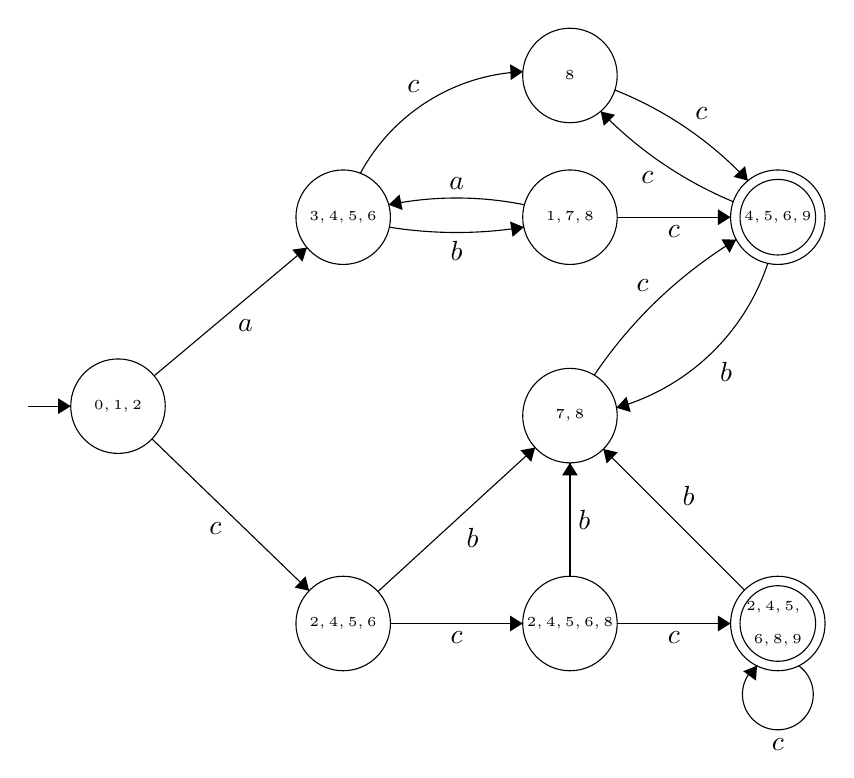
\begin{tikzpicture}[scale=0.2]
                \tikzstyle{every node}+=[inner sep=0pt]
                \draw [black] (10.8,-24.8) circle (3);
                \draw (10.8,-24.8) node {\tiny $0,1,2$};
                \draw [black] (25.1,-12.8) circle (3);
                \draw (25.1,-12.8) node {\tiny $3,4,5,6$};
                \draw [black] (39.5,-12.8) circle (3);
                \draw (39.5,-12.8) node {\tiny $1,7,8$};
                \draw [black] (52.7,-12.8) circle (3);
                \draw (52.7,-12.8) node {\tiny $4,5,6,9$};
                \draw [black] (52.7,-12.8) circle (2.4);
                \draw [black] (39.5,-3.8) circle (3);
                \draw (39.5,-3.8) node {\tiny $8$};
                \draw [black] (39.5,-25.4) circle (3);
                \draw (39.5,-25.4) node {\tiny $7,8$};
                \draw [black] (25.1,-38.6) circle (3);
                \draw (25.1,-38.6) node {\tiny $2,4,5,6$};
                \draw [black] (39.5,-38.6) circle (3);
                \draw (39.5,-38.6) node {\tiny $2,4,5,6,8$};
                \draw [black] (52.7,-38.6) circle (3);
                \draw (52.7,-38.6) node[text width = 0.8cm, 
                                        align = center] {\tiny $2,4,5,\newline 6,8,9$};
                \draw [black] (52.7,-38.6) circle (2.4);
                \draw [black] (5.1,-24.8) -- (7.8,-24.8);
                \fill [black] (7.8,-24.8) -- (7,-24.3) -- (7,-25.3);
                \draw [black] (13.1,-22.87) -- (22.8,-14.73);
                \fill [black] (22.8,-14.73) -- (21.87,-14.86) -- (22.51,-15.63);
                \draw (18.9,-19.29) node [below] {$a$};
                \draw [black] (36.569,-13.434) arc (-80.95264:-99.04736:27.15);
                \fill [black] (36.57,-13.43) -- (35.7,-13.07) -- (35.86,-14.05);
                \draw (32.3,-14.27) node [below] {$b$};
                \draw [black] (27.991,-12.009) arc (101.37485:78.62515:21.847);
                \fill [black] (27.99,-12.01) -- (28.87,-12.34) -- (28.68,-11.36);
                \draw (32.3,-11.08) node [above] {$a$};
                \draw [black] (42.5,-12.8) -- (49.7,-12.8);
                \fill [black] (49.7,-12.8) -- (48.9,-12.3) -- (48.9,-13.3);
                \draw (46.1,-13.3) node [below] {$c$};
                \draw [black] (26.191,-10.013) arc (151.63687:92.3739:12.314);
                \fill [black] (36.52,-3.56) -- (35.7,-3.09) -- (35.74,-4.09);
                \draw (29.56,-4.92) node [above] {$c$};
                \draw [black] (42.352,-4.724) arc (68.35935:43.0669:23.346);
                \fill [black] (50.8,-10.48) -- (50.62,-9.56) -- (49.89,-10.24);
                \draw (47.84,-6.64) node [above] {$c$};
                \draw [black] (12.96,-26.88) -- (22.94,-36.52);
                \fill [black] (22.94,-36.52) -- (22.71,-35.6) -- (22.02,-36.32);
                \draw (16.99,-32.18) node [below] {$c$};
                \draw [black] (27.31,-36.57) -- (37.29,-27.43);
                \fill [black] (37.29,-27.43) -- (36.36,-27.6) -- (37.04,-28.34);
                \draw (33.31,-32.49) node [below] {$b$};
                \draw [black] (41.044,-22.829) arc (146.05367:121.28189:29.056);
                \fill [black] (50.06,-14.22) -- (49.12,-14.21) -- (49.64,-15.07);
                \draw (44.12,-17.55) node [above] {$c$};
                \draw [black] (52.064,-15.726) arc (-18.33145:-74.33299:14.151);
                \fill [black] (42.45,-24.9) -- (43.36,-25.17) -- (43.09,-24.2);
                \draw (49.42,-21.99) node [below] {$b$};
                \draw [black] (28.1,-38.6) -- (36.5,-38.6);
                \fill [black] (36.5,-38.6) -- (35.7,-38.1) -- (35.7,-39.1);
                \draw (32.3,-39.1) node [below] {$c$};
                \draw [black] (42.5,-38.6) -- (49.7,-38.6);
                \fill [black] (49.7,-38.6) -- (48.9,-38.1) -- (48.9,-39.1);
                \draw (46.1,-39.1) node [below] {$c$};
                \draw [black] (54.023,-41.28) arc (54:-234:2.25);
                \draw (52.7,-45.85) node [below] {$c$};
                \fill [black] (51.38,-41.28) -- (50.5,-41.63) -- (51.31,-42.22);
                \draw [black] (39.5,-35.6) -- (39.5,-28.4);
                \fill [black] (39.5,-28.4) -- (39,-29.2) -- (40,-29.2);
                \draw (40,-32) node [right] {$b$};
                \draw [black] (50.58,-36.48) -- (41.62,-27.52);
                \fill [black] (41.62,-27.52) -- (41.83,-28.44) -- (42.54,-27.73);
                \draw (46.62,-30.52) node [right] {$b$};
                \draw [black] (49.868,-11.815) arc (-112.60551:-135.96825:25.156);
                \fill [black] (41.45,-6.08) -- (41.65,-7) -- (42.37,-6.3);
                \draw (44.42,-9.87) node [below] {$c$};
            \end{tikzpicture}
        \end{center}
    \end{solution}

    \part Give a regular expression that defines the same language as
    this NFA.
    \begin{solution}
        \[
            (
                (a(ba)^\star) 
                \mid 
                (cc^\star)
            )
            (
                (b \mid c)
                c
            )^\star.
        \]
    \end{solution}
\end{parts}

\question In the lecture we saw the following transition diagram
for identifies (\textbf{id}'s):
\begin{center}
    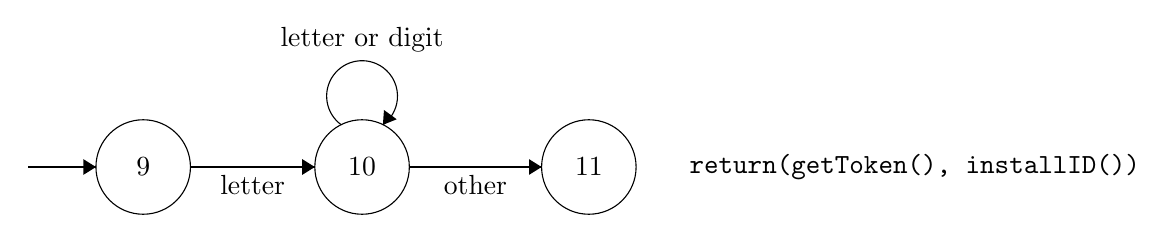
\begin{tikzpicture}[scale=0.2]
        \tikzstyle{every node}+=[inner sep=0pt]
        \draw [black] (16,-24.9) circle (3);
        \draw (16,-24.9) node {$9$};
        \draw [black] (29.9,-24.9) circle (3);
        \draw (29.9,-24.9) node {$10$};
        \draw [black] (44.3,-24.9) circle (3);
        \draw (44.3,-24.9) node {$11$};
        \draw [black] (19,-24.9) -- (26.9,-24.9);
        \fill [black] (26.9,-24.9) -- (26.1,-24.4) -- (26.1,-25.4);
        \draw (22.95,-25.4) node [below] {letter};
        \draw [black] (28.577,-22.22) arc (234:-54:2.25);
        \draw (29.9,-17.65) node [above] {letter or digit};
        \fill [black] (31.22,-22.22) -- (32.1,-21.87) -- (31.29,-21.28);
        \draw [black] (32.9,-24.9) -- (41.3,-24.9);
        \fill [black] (41.3,-24.9) -- (40.5,-24.4) -- (40.5,-25.4);
        \draw (37.1,-25.4) node [below] {other};
        \draw [black] (8.7,-24.9) -- (13,-24.9);
        \fill [black] (13,-24.9) -- (12.2,-24.4) -- (12.2,-25.4);
        \draw (65, -24.9) node {\texttt{return(getToken(), installID())}};
    \end{tikzpicture}
\end{center}
\begin{parts}
    \part Design a transition diagram for unsigned decimal numbers,
    for instance $143.7897$ or $23.9808$.
    \begin{solution}
        \begin{center}
            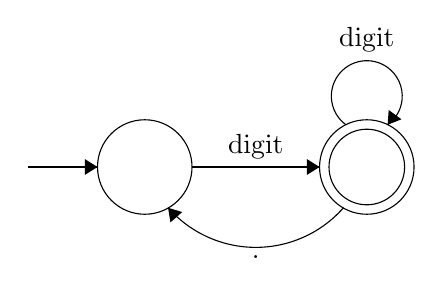
\begin{tikzpicture}[scale=0.2]
                \tikzstyle{every node}+=[inner sep=0pt]
                \draw [black] (16.4,-25.9) circle (3);
                \draw [black] (30.5,-25.9) circle (3);
                \draw [black] (30.5,-25.9) circle (2.4);
                \draw [black] (9,-25.9) -- (13.4,-25.9);
                \fill [black] (13.4,-25.9) -- (12.6,-25.4) -- (12.6,-26.4);
                \draw [black] (19.4,-25.9) -- (27.5,-25.9);
                \fill [black] (27.5,-25.9) -- (26.7,-25.4) -- (26.7,-26.4);
                \draw (23.45,-25.4) node [above] {digit};
                \draw [black] (29.177,-23.22) arc (234:-54:2.25);
                \draw (30.5,-18.65) node [above] {digit};
                \fill [black] (31.82,-23.22) -- (32.7,-22.87) -- (31.89,-22.28);
                \draw [black] (29.02,-28.486) arc (-41.35346:-138.64654:7.421);
                \fill [black] (17.88,-28.49) -- (18.03,-29.42) -- (18.78,-28.76);
                \draw (23.45,-31.5) node [below] {.};
            \end{tikzpicture}
        \end{center}
    \end{solution}

    \part Extend the transition diagram of question (a), such that
    it recognises also unsigned decimal numbers that are followed
    by (optional) exponents, for instance
    \texttt{12.5989E34} (which can be met also as \texttt{12.5989E+34}
    and it means $12.5989\cdot 10^3$)
    or \texttt{23.132E-2} (which means $23.132\cdot 10^{-2}$).
    \begin{solution}
        \begin{center}
            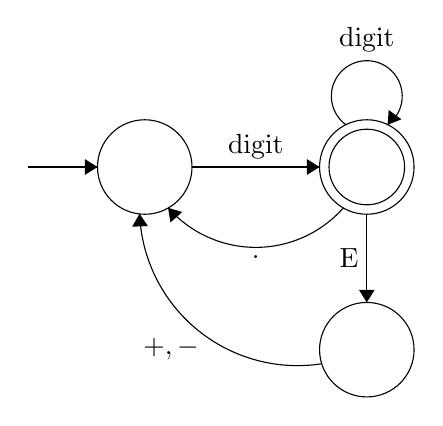
\begin{tikzpicture}[scale=0.2]
                \tikzstyle{every node}+=[inner sep=0pt]
                \draw [black] (16.4,-25.9) circle (3);
                \draw [black] (30.5,-25.9) circle (3);
                \draw [black] (30.5,-25.9) circle (2.4);
                \draw [black] (30.5,-37.5) circle (3);
                \draw [black] (9,-25.9) -- (13.4,-25.9);
                \fill [black] (13.4,-25.9) -- (12.6,-25.4) -- (12.6,-26.4);
                \draw [black] (19.4,-25.9) -- (27.5,-25.9);
                \fill [black] (27.5,-25.9) -- (26.7,-25.4) -- (26.7,-26.4);
                \draw (23.45,-25.4) node [above] {digit};
                \draw [black] (29.177,-23.22) arc (234:-54:2.25);
                \draw (30.5,-18.65) node [above] {digit};
                \fill [black] (31.82,-23.22) -- (32.7,-22.87) -- (31.89,-22.28);
                \draw [black] (29.02,-28.486) arc (-41.35346:-138.64654:7.421);
                \fill [black] (17.88,-28.49) -- (18.03,-29.42) -- (18.78,-28.76);
                \draw (23.45,-31.5) node [below] {.};
                \draw [black] (30.5,-28.9) -- (30.5,-34.5);
                \fill [black] (30.5,-34.5) -- (31,-33.7) -- (30,-33.7);
                \draw (30,-31.7) node [left] {E};
                \draw [black] (27.648,-38.394) arc (-81.15355:-177.73437:10.04);
                \fill [black] (16.07,-28.87) -- (15.6,-29.69) -- (16.6,-29.65);
                \draw (18.07,-36.72) node [below] {$+,-$};
            \end{tikzpicture}
        \end{center}
    \end{solution}
\end{parts}

\question In the lecture we saw how the software tool
Lex performs pattern matching.
Assume that Lex has the following patterns in this order:
\begin{enumerate}
    \item $ab$;
    \item $a^\star b$; and
    \item $(a \mid b)^\star b$.
\end{enumerate}
Build the NFA that Lex would use for these patterns.
\begin{solution}
    \begin{center}
        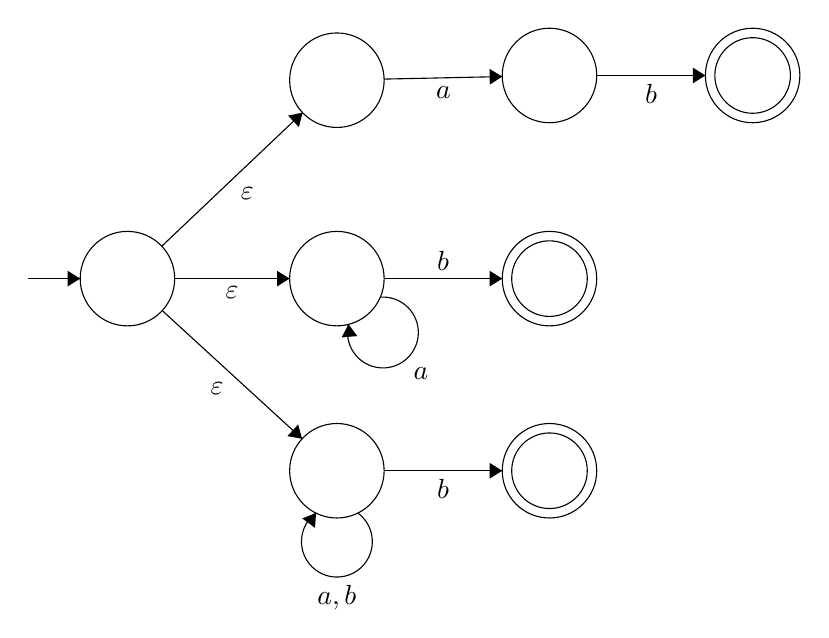
\begin{tikzpicture}[scale=0.2]
            \tikzstyle{every node}+=[inner sep=0pt]
            \draw [black] (10.9,-24.4) circle (3);
            \draw [black] (24.2,-11.8) circle (3);
            \draw [black] (24.2,-24.4) circle (3);
            \draw [black] (24.2,-36.6) circle (3);
            \draw [black] (37.7,-11.5) circle (3);
            \draw [black] (50.6,-11.5) circle (3);
            \draw [black] (50.6,-11.5) circle (2.4);
            \draw [black] (37.7,-24.4) circle (3);
            \draw [black] (37.7,-24.4) circle (2.4);
            \draw [black] (37.7,-36.6) circle (3);
            \draw [black] (37.7,-36.6) circle (2.4);
            \draw [black] (4.6,-24.4) -- (7.9,-24.4);
            \fill [black] (7.9,-24.4) -- (7.1,-23.9) -- (7.1,-24.9);
            \draw [black] (13.9,-24.4) -- (21.2,-24.4);
            \fill [black] (21.2,-24.4) -- (20.4,-23.9) -- (20.4,-24.9);
            \draw (17.55,-24.9) node [below] {$\varepsilon$};
            \draw [black] (13.11,-26.43) -- (21.99,-34.57);
            \fill [black] (21.99,-34.57) -- (21.74,-33.66) -- (21.06,-34.4);
            \draw (16.59,-30.99) node [below] {$\varepsilon$};
            \draw [black] (13.08,-22.34) -- (22.02,-13.86);
            \fill [black] (22.02,-13.86) -- (21.1,-14.05) -- (21.79,-14.78);
            \draw (18.51,-18.58) node [below] {$\varepsilon$};
            \draw [black] (25.523,-39.28) arc (54:-234:2.25);
            \draw (24.2,-43.85) node [below] {$a,b$};
            \fill [black] (22.88,-39.28) -- (22,-39.63) -- (22.81,-40.22);
            \draw [black] (27.2,-36.6) -- (34.7,-36.6);
            \fill [black] (34.7,-36.6) -- (33.9,-36.1) -- (33.9,-37.1);
            \draw (30.95,-37.1) node [below] {$b$};
            \draw [black] (26.946,-25.578) arc (94.50925:-193.49075:2.25);
            \draw (29.54,-30.02) node [below] {$a$};
            \fill [black] (24.94,-27.3) -- (24.5,-28.13) -- (25.5,-28.05);
            \draw [black] (27.2,-24.4) -- (34.7,-24.4);
            \fill [black] (34.7,-24.4) -- (33.9,-23.9) -- (33.9,-24.9);
            \draw (30.95,-23.9) node [above] {$b$};
            \draw [black] (27.2,-11.73) -- (34.7,-11.57);
            \fill [black] (34.7,-11.57) -- (33.89,-11.08) -- (33.91,-12.08);
            \draw (30.96,-12.17) node [below] {$a$};
            \draw [black] (40.7,-11.5) -- (47.6,-11.5);
            \fill [black] (47.6,-11.5) -- (46.8,-11) -- (46.8,-12);
            \draw (44.15,-12) node [below] {$b$};
        \end{tikzpicture}
    \end{center}
\end{solution}
Then, provide the patterns that would be returned by Lex
with the following strings as inputs, as well as the longest
matched prefixes:
\begin{parts}
    \part $ab$;
    \part $abab$;
    \part $aab$; and
    \part $aaba$.
\end{parts}
\begin{solution}
    Lex would return:
    \begin{enumerate}
        \item $ab$;
        \item $(a \mid b)^\star b$;
        \item $a^\star b$; and
        \item $a^\star b$.
    \end{enumerate}
\end{solution}
